% -*-latex-*-
\documentclass[pdftex,12pt]{beamer}
\usepackage{etex,pictex,color}
\usepackage{graphicx}
\usepackage{pbox}
\usepackage{bbding}
\usepackage{ifthen}
\newcounter{showthis}
\setcounter{showthis}{1}
\setbeamercovered{transparent}
\setbeamertemplate{footline}[frame number]
\begin{document}
\title{The Nature of Neanderthal Introgression Revealed by 27,566
  Icelandic Genomes}
\author{Laurits Skov et al}
\date{22 April 2020}

\frame{\titlepage}

\begin{frame}
  \frametitle{Overview}
  Used a 2-state hidden Markov model (not conditioned on archaic
  genomes) to search for archaic haplotypes in 55,132 Icelandic
  haploid genomes sequenced to 30X.

  \bigskip

  Found 112,709 archaic haplotypes covering 1.179~Gb, or 48.2\% of the
  callable genome.

  \bigskip

  These introgressed fragments cover 1.34\% of the average Icelandic
  genome---an underestimate, because the method can detect
  introgressed fragments only if they are sufficiently long and
  sufficiently divergent. Estimated false-negative rate suggests a
  true fraction closer to 1.9\%.

\end{frame}

\begin{frame}
  \frametitle{Multiple archaic sources}
  \begin{center}
  \begin{tabular}{lr}
    Neanderthal & 84.5\%\\
    Denisovan   & 3.3\%\\
    Unknown     & 12.2\%\\
  \end{tabular}
  \end{center}
The Denisovan fraction is larger than expected through incomplete
lineage sorting. Suggests Denisovan gene flow either via Neanderthals
or directly into moderns.
\end{frame}

\begin{frame}
  \frametitle{Mosaic haplotypes}

  18.9\% of archaic haplotypes were ``mosaic,'' including Denisovan as
  well as Neanderthal variants.

  \bigskip

  This is remarkable. The authors discuss two hypotheses:
  (1)~Denisovans interbred with Neanderthals, who later interbred with
  moderns, or (2)~Denisovans interbred directly with moderns.

  \bigskip

  The first hypothesis seems more plausible, because we know there was
  interbreeding between N and D. Furthermore, the fraction of archaic
  DNA in moderns is low, and this would have reduced the opportunity
  for recombinant N-D haplotypes to form.

\end{frame}

\begin{frame}
  \frametitle{Models of history}
  \centering
  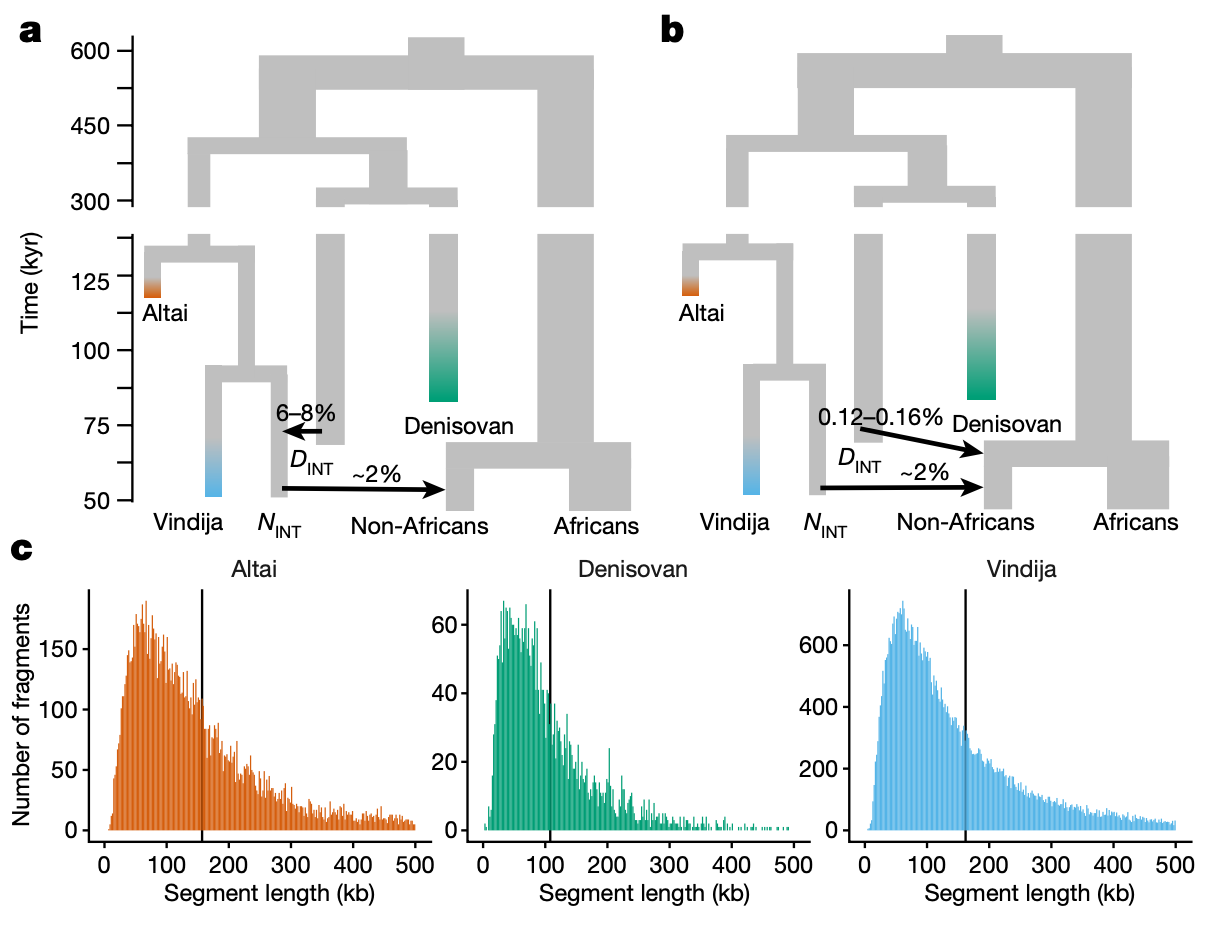
\includegraphics[width=\linewidth]{networks}\\
\end{frame}  

\begin{frame}
  \frametitle{Population size estimates}

  Archaic population sizes were estimated by comparing introgressed
  haplotypes with the sequences of archaic genomes.

  \bigskip

  Estimate small $N_e$ for both archaics: 2000--3000 individuals.

  \bigskip

  I don't fully understand what they did and have been emailing with
  the authors.

\end{frame}

\begin{frame}
  \frametitle{Distribution of archaic DNA w/i the modern genome}

  I don't entirely understand the prose, but I think it says that
  archaic DNA is more common where recombination rate is high.

  \bigskip

  This is interesting, because archaic haplotypes should be shorter in
  these regions and thus more difficult to detect.

  \bigskip

  Implies that archaic variants are more likely to survive if they can
  be uncoupled from deleterious archaic variants.
\end{frame}

\begin{frame}
  \frametitle{Mutational bias}
  \begin{columns}
    \column{0.5\textwidth}
    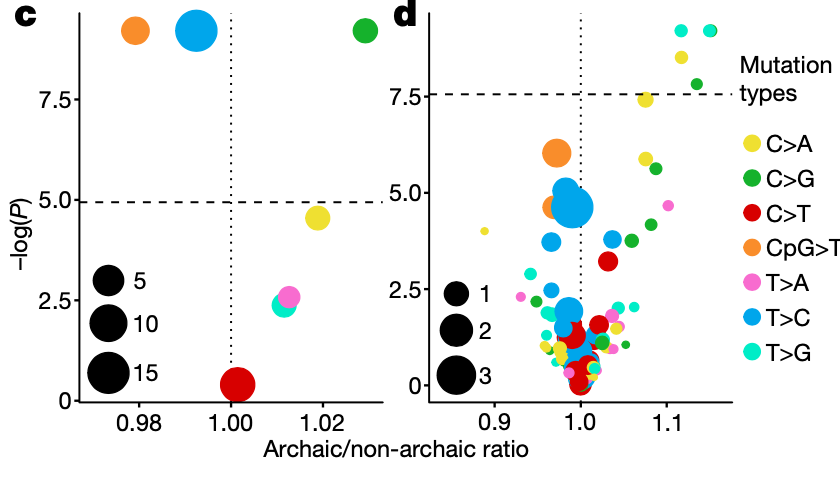
\includegraphics[width=\linewidth]{muttype.png}
    \column{0.5\textwidth}
    \raggedleft
    Archaics and moderns have similar mutation rates.

    \bigskip

    But they differ in the frequencies of different categories of
    mutation.

    \bigskip

    The largest differences may reflect differences between the two
    populations in the average ages of mothers and fathers.
  \end{columns}

\end{frame}

\begin{frame}
  \frametitle{No evidence of selection against archaic DNA}
  \begin{columns}
    \column{0.5\textwidth}
    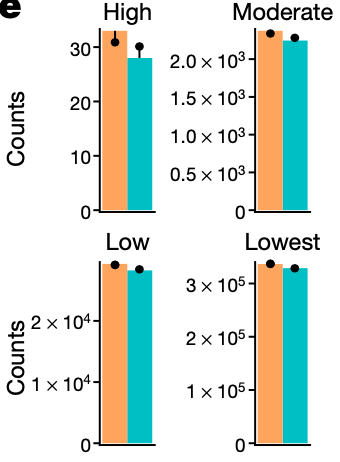
\includegraphics[width=\linewidth]{noseln.png}
    \column{0.5\textwidth}
    \raggedleft

    No excess of deleterious variants in archaic haplotypes.

    \bigskip

    Yet abundant evidence shows that archaic genomes had lots of
    deleterious variants.

    \bigskip

    Presumably, these were removed in moderns by purifying selection.
  \end{columns}

\end{frame}

\begin{frame}
  \frametitle{Effects on function}

  Looked for associations between archaic haplotypes and 271
  phenotypes.

  \bigskip

  Removed associations that were better explained by a nearby
  non-archaic site.

  \bigskip

  Pooled linked archaic haplotypes

  \bigskip

  After filtering, only 5 archaic associations remained.

  \bigskip

  Verify only 3 of 26 previously-reported archaic associations.

  \bigskip

  Neither was there a significant association between any of the
  phenotypes and the \emph{number} of archaic haplotypes.

\end{frame}

\begin{frame}
  \frametitle{Discussion questions}
  \begin{enumerate}
    \item How might we distinguish between the two hypotheses to
      explain the presence of Denisovan DNA and Neanderthal-Denisovan
      mosaics? 
    \item Are we convinced by the argument that archaic DNA doesn't
      affect function?
    \item What might explain the apparent difference in average ages
      of mothers and fathers?
  \end{enumerate}
\end{frame}

\end{document}


